\subsubsection{Typische Komponenten und Bauweisen analoger Computer}
\label{chap:Typische Komponenten und Bauweisen analoger Computer}

Der Operationsverstärker gilt als zentraler Baustein für die meisten Komponenten eines analogen Rechners. Er bildet die Differenz aus zwei Eingangssignalen und verstärkt dieses Signal anschließend. Werden ein freies und ein geerdetes Eingangssignal genutzt, so wird nur das Freie verstärkt. Durch ein Rückkopplungs-Signal gelingt es dem Operationsverstärker einen Teil der Stromverstärkung aufzugeben, um Stabilität zu gewinnen. Dieses Signal verbindet die Ausgabe der Komponente mit seiner Eingabe, wobei diese beiden Werte miteinander summiert werden. Ein wichtiges Merkmal dieser Komponente ist außerdem, dass das Vorzeichen der Eingabe gedreht wird. (\cite[vgl. S. 73 f.]{Ulmann2022})

\begin{figure}[h]
  \label{fig:Operationsverstärker mit Rückkopplung}
  \caption{Operationsverstärker mit Rückkopplung}
  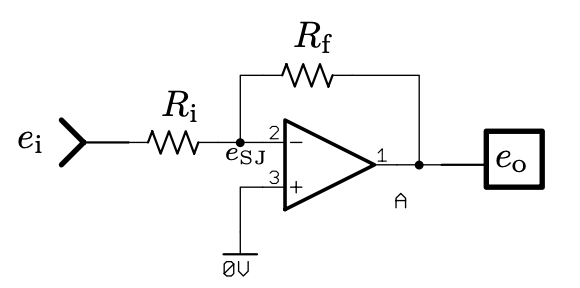
\includegraphics[width=0.5\textwidth]{abbildungen/opamp_mit_rueckkopplung.png}
  \\
  Quelle: \cite[S. 76]{Ulmann2022}
\end{figure}

Die Formel zu Berechnung der Ausgangsspannung lautet damit wie folgt:

\[e_o=\frac{R_f}{R_i}e_i\]

Durch Anpassungen des Eingangssignals bzw. des Rückkopplungs-Signals kann die Funktion des Operationsverstärkers geändert werden. So sind hiermit Operationen wie Summieren, Subtrahieren, Invertieren, das Multiplizieren von Konstanten, Integration und (bedingt) die Differenzierung möglich.

Im Prozess der Verstärkung der Signale kann ein sog. Drift auftreten. Dadurch werden kleine Fehler in der Signalverarbeitung verstärkt und führen zu großen Fehlern am Ausgang. Dieses Problem kann durch Drift-Stabilisierung gelöst werden, wie beschrieben in einem Patent von \cite{Goldberg1954}. Das durch Drift verursachte Fehlersignal kann an der Summe des Eingangs- und Rückkopplungs-Signals ausgelesen werden. Es wird verstärkt und als weiteres Eingangssignal genutzt. Somit wird der Drift ausgeglichen. (\cite[vgl. S. 80]{Ulmann2022})

Um einen Summierer zu bilden, muss lediglich ein weiteres Eingangssignal zum Operationsverstärker hinzugefügt werden. Die Widerstände \(R_i\) bilden die Koeffizienten der Eingangssignale. Der Summierer bildet also die gewichtete Summe der Eingangssignale und gibt diese invertiert aus. (\cite[vgl. S. 86]{Ulmann2022})

Wird der Feedback-Widerstand \(R_f\) durch einen Kondensator \(C\) ersetzt, wird die Summe der Eingangssignale über Zeit integriert. Man erhält also einen Integrierer. Durch ein Steuerelement \textit{IC} wird ein Initialwert festgelegt, der so lange ausgegeben wird, bis ein weiteres Steuerelement \textit{OP} betätigt wird. Im aktivierten Zustand wird so lange das Integral der Eingangssignale ausgegeben, bis der \textit{OP} Schalter erneut betätigt und der letzte gespeicherte Wert ausgegeben wird. (\cite[vgl. S. 89 ff.]{Ulmann2022})

Die Anwendung eines Koeffizienten am Operationsverstärker kann durch ein Potentiometer erfolgen, welches am Eingangssignal angeschlossen ist. Das somit erhaltene Koeffizient-Potentiometer lässt sich über einen speziellen Zustand des Analogrechners, dem \textit{Potentiometer Set} (kurz: \textit{Pot Set}) setzen. In diesem Zustand werden alle Recheneinheiten des Analogrechners deaktiviert, sodass das rohe Eingangssignal weitergeleitet wird. In großen analogen Rechnern werden Potentiometer durch Servomotoren oder in hybriden Rechnern digital gesteuert. (\cite[vgl. S. 92 ff.]{Ulmann2022})

Ein Funktionsgenerator kann genutzt werden, um eine beliebige Funktion \(f(x,...)\) abzubilden. Für analoge Rechner ist das aber eine komplexe Aufgabe, weshalb sich für diesen Anwendungsfall hybride Systeme besonders eignen. Als mögliche analoge Ansätze bieten sich der servogetriebene Funktionsgenerator, der Kurvenfolger oder der Fotoformer an (\cite[vgl. S. 97 ff.]{Ulmann2022}).

\begin{figure}[h]
  \label{fig:Symbole analoger Computer}
  \caption{Symbole zur Darstellung eines analogen Computers}
  \centering
  \begin{subfigure}[b]{0.2\textwidth}
    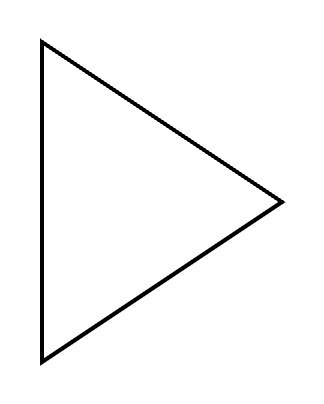
\includegraphics[width=\textwidth]{abbildungen/symbol_summierer.png}
    \caption{Summierer}
  \end{subfigure}%
  \hfill
  \begin{subfigure}[b]{0.2\textwidth}
    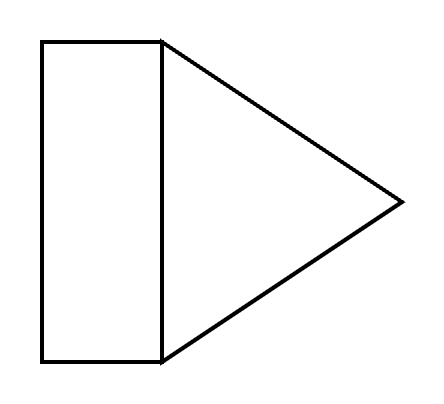
\includegraphics[width=\textwidth]{abbildungen/symbol_integrierer.png}
    \caption{Integrierer}
  \end{subfigure}%
  \hfill
  \begin{subfigure}[b]{0.2\textwidth}
    
\includegraphics[width=\textwidth]{abbildungen/symbol_potentiometer.png}
    \caption{Potentiometer}
  \end{subfigure}%
  \hfill
  \begin{subfigure}[b]{0.2\textwidth}
    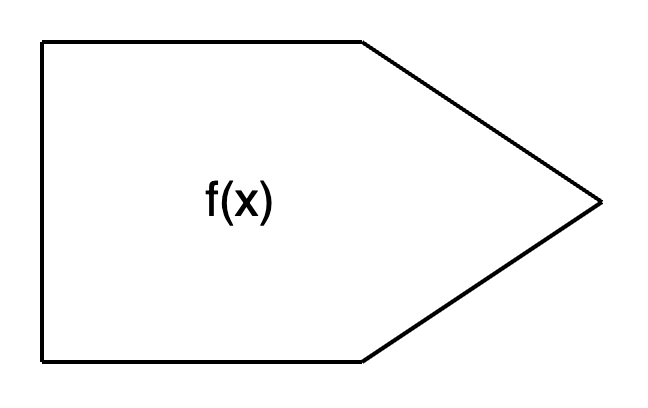
\includegraphics[width=\textwidth]{abbildungen/symbol_funktionsgenerator.png}
    \caption{Funktionsgenerator}
  \end{subfigure}
  \\
  Quelle: Eigene Darstellung
\end{figure}

Die im ersten Augenblick einfache Multiplizierung ist auf analogen Rechnern komplex zu implementieren (\cite[vgl. S. 105]{Ulmann2022}). Moderne analoge Rechner greifen typischerweise auf die Gilbert Zelle zurück. Die Berechnung einer Division bzw. Quadratwurzel kann durch modifizierte Multiplikatoren erfolgen. (\cite[S. 114 f.]{Ulmann2022})

Ein Komparator kann \zb zur Implementierung einer Schrittfunktion oder zum Tauschen von Variablen genutzt werden. Um das zu erreichen, reicht es schon aus, Dioden in der Feedback-Schleife eines Operationsverstärkers zu platzieren. Nach einem ähnlichen Prinzip kann auch ein Begrenzer erzeugt werden, dessen Eingangssignal zwischen einer Ober- und Untergrenze limitiert wird. (\cite[S. 116]{Ulmann2022})

Die im Jahr 2020 gegründete anabrid GmbH hat es sich zum Ziel gesetzt, analoge und digitale Technologien zu kombinieren, um die technologischen Herausforderungen der Zukunft effizient lösen zu können. Dazu entwickelt und vertreibt das Unternehmen rekonfigurierbare analoge Rechner, wie den 2024 erschienenen "`lucidac"' oder das rudimentäre "`The Analog Thing"' (\cite{AnabridWebsite}).

\begin{quote}
  "`THE ANALOG THING is a high-quality, low-cost, open-source, and not-for-profit cutting-edge analog computer. You can think of it as a kind of Raspberry Pi that computes with continuous voltages rather than with zeroes and ones."' (\cite{TheAnalogThingDocs})
\end{quote}

Das \ac{that} orientiert sich am historischen Design der analogen Computer und arbeitet demnach mit Patchkabeln, mit denen Rechenelemente verschaltet werden (siehe Abbildung \ref{fig:The Analog Thing}). Dabei arbeitet das Gerät mit 10 Volt und in einem Wertebereich von \pm 1. Fällt eine Spannung außerhalb dieses Wertebereichs, fällt das Gerät in den sog. "`Overload"'-Modus und signalisiert dies über eine LED. Außerdem bietet das Gerät Anschlüsse für einige Variablen, welche als Ein- oder Ausgaben zur Auswertung oder Verschaltung mit weiteren analogen Rechnern genutzt werden können (\cite{TheAnalogThingDocs}).

\begin{figure}[h]
  \label{fig:The Analog Thing}
  \caption{The Analog Thing des Herstellers anabrid GmbH}
  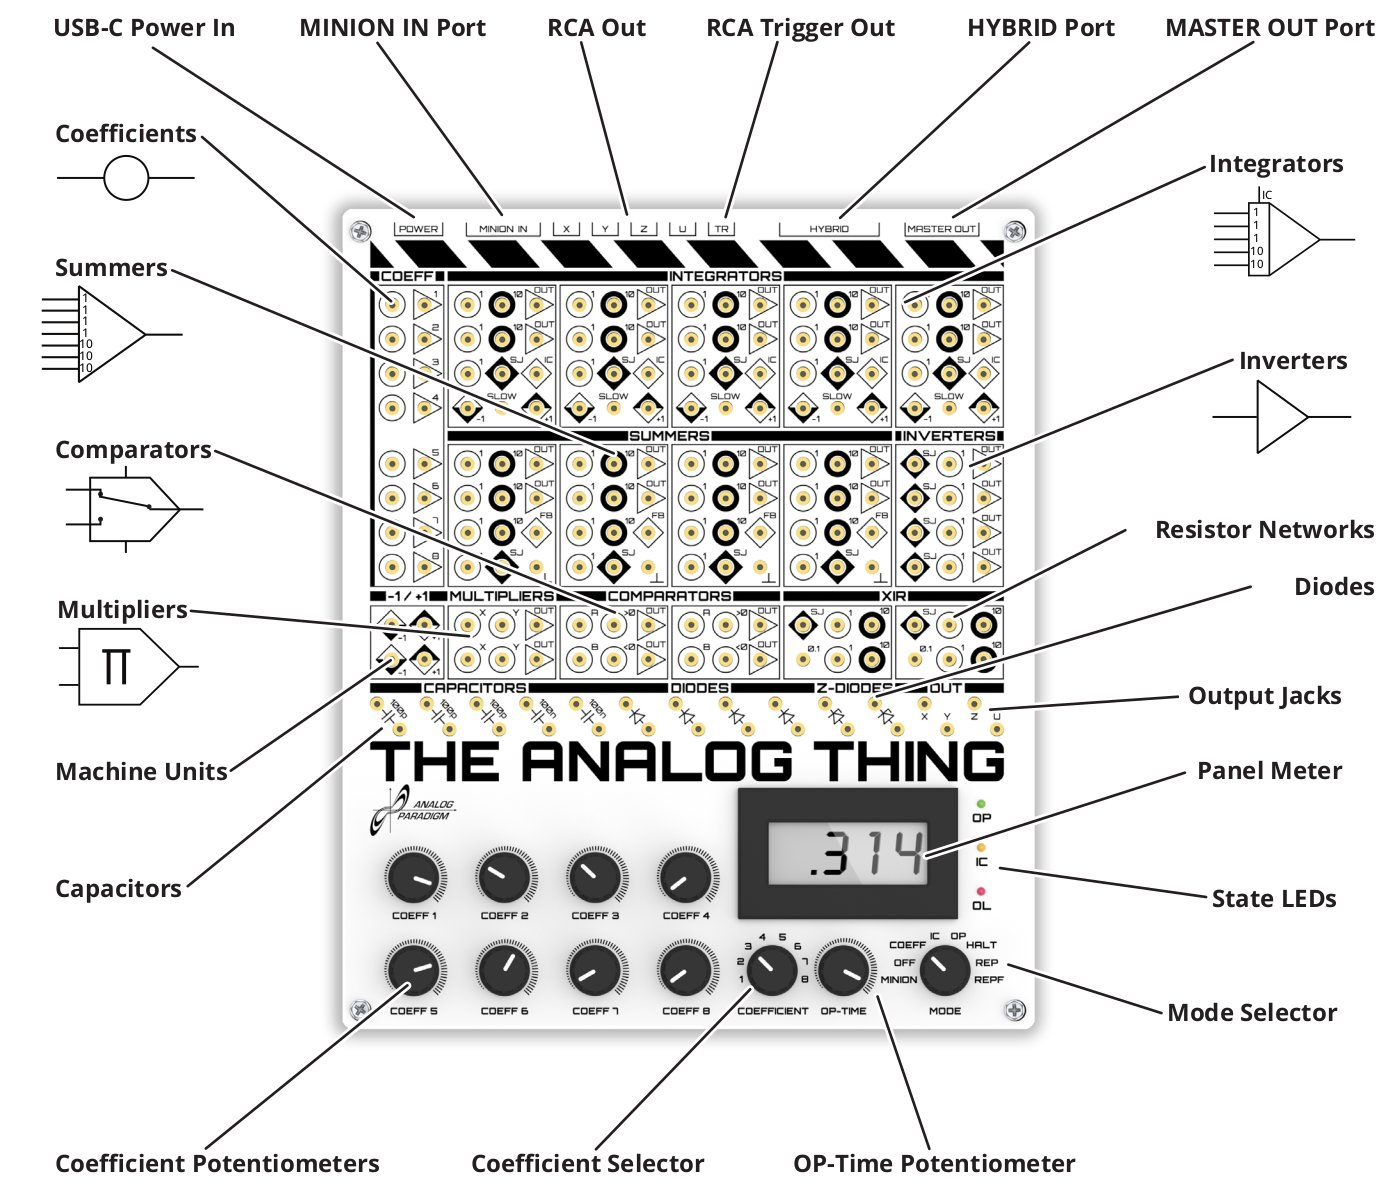
\includegraphics[width=0.75\textwidth]{abbildungen/the_analog_thing.jpg}
  \\
  Quelle: \cite{TheAnalogThingDocs}
\end{figure}

Wie in Abbildung \ref{fig:The Analog Thing} zu sehen, bietet das \ac{that} die grundlegenden Komponenten wie Potentiometer, Summierer, Integrierer, Multiplizierer und Komparatoren an. Diese Komponenten reichen bereits aus, um Probleme wie die Euler-Spirale zu lösen (Siehe Abbildung \ref{fig:THAT Euler Spirale})

\begin{figure}[h]
  \label{fig:THAT Euler Spirale}
  \caption{Simulation der Euler-Spirale auf einem \ac{that}}
  \begin{subfigure}{.2\textwidth}
    \centering
    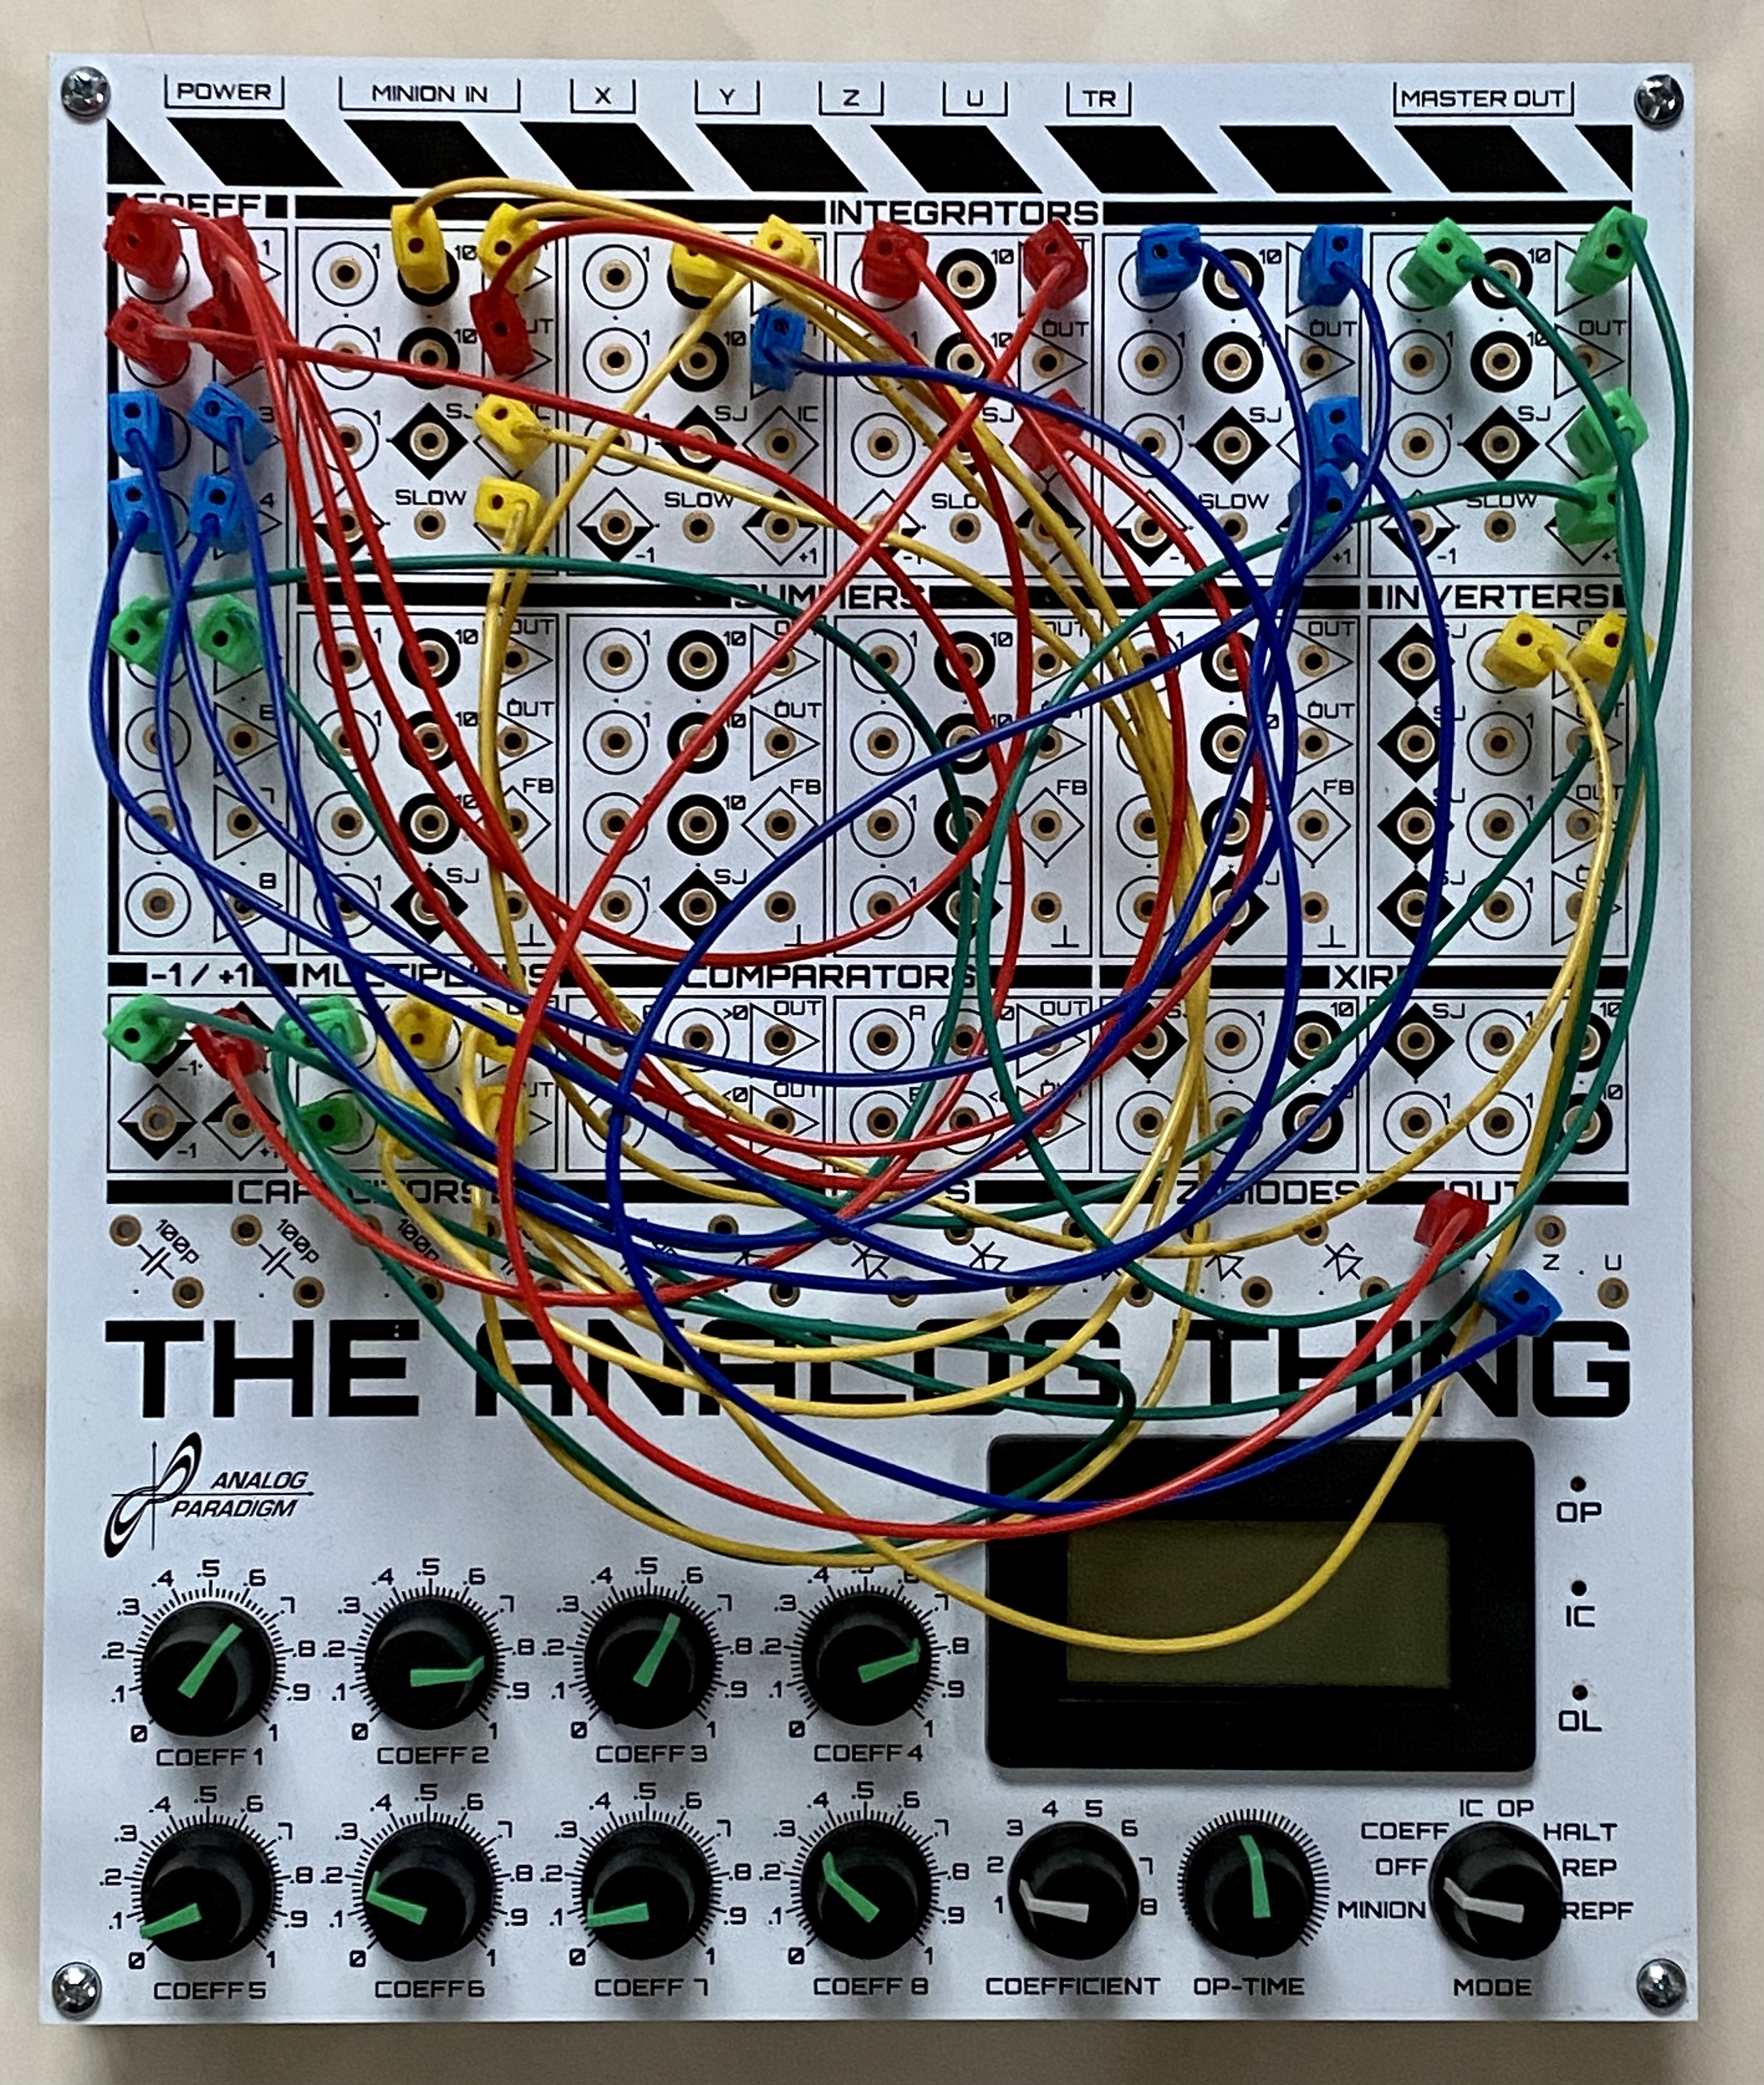
\includegraphics[width=\textwidth]{abbildungen/euler_spirale_implementierung.jpg}\par
  \end{subfigure}
  \begin{subfigure}{.2\textwidth}
    \centering
    
\includegraphics[width=\textwidth]{abbildungen/euler_spirale_ausgabe.jpg}\par
  \end{subfigure}
  \\
  Quelle: \cite{TheAnalogThingDocs}
\end{figure}

Das neueste Modell des Herstellers Anabrid, der "`lucidac"', lasst sich digital über Software progammieren, wodurch der manuelle Aufwand durch die Verkabelung des Rechners wegfällt (\cite[vgl.]{AnabridLucidAC2025}). Dafür wurde eine Python-Bibliothek entwickelt, die durch Befehle wie "`connect(a, b)"' Verbindungen zwischen Komponenten herstellen kann (\cite[vgl.]{AnabridLucipy}). Um die software-gesteuerte Programmierung zu ermöglichen, verwendet der lucidac eine Verbindungs-Matrix, welche der Verbindung aller Komponenten ein Gewicht zuweist. Wird ein Wert innerhalb der Matrix von null auf \zb eins geändert, so wird eine neue (gewichtete) Verbindung hergestellt (\cite{AnabridLucidAC2025}). Seien \(C^{in}\) bzw. \(C^{out}\) die Ein- bzw. Ausgaben der Komponenten und \(M\) die gewichteten Verbindung zwischen Komponenten, so gilt:

\[C_i^{in}=\sum_{j=0}^{16}M_{ij}C_j^{out}, i,j\in[0,16]\]
